\documentclass{extbook}[14pt]
\usepackage{multicol, enumerate, enumitem, hyperref, color, soul, setspace, parskip, fancyhdr, amssymb, amsthm, amsmath, bbm, latexsym, units, mathtools}
\everymath{\displaystyle}
\usepackage[headsep=0.5cm,headheight=0cm, left=1 in,right= 1 in,top= 1 in,bottom= 1 in]{geometry}
\pagestyle{fancy}
\lhead{}
\chead{Answer Key for Module\,6\,-\,Polynomial\,Functions Version C}
\rhead{}
\lfoot{Summer\,C\,2020}
\cfoot{}
\rfoot{}
\begin{document}
\textbf{This key should allow you to understand why you choose the option you did (beyond just getting a question right or wrong). \href{https://xronos.clas.ufl.edu/mac1105spring2020/courseDescriptionAndMisc/Exams/LearningFromResults}{More instructions on how to use this key can be found here}.}

\textbf{If you have a suggestion to make the keys better, \href{https://forms.gle/CZkbZmPbC9XALEE88}{please fill out the short survey here}.}

\textit{Note: This key is auto-generated and may contain issues and/or errors. The keys are reviewed after each exam to ensure grading is done accurately. If there are issues (like duplicate options), they are noted in the offline gradebook. The keys are a work-in-progress to give students as many resources to improve as possible.}

\rule{\textwidth}{0.4pt}

1. Describe the end behavior of the polynomial below.
\[ f(x) = -8(x + 8)^{2}(x - 8)^{5}(x - 4)^{4}(x + 4)^{6} \] 

 
 The solution is  
 \begin{center} 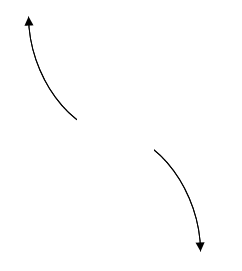
\includegraphics[width=0.3\textwidth]{../Figures/polyEndBehaviorAC.png} \end{center}\begin{tabular}{|c|c|} 
\hline 
 & \tabularnewline 
 \textbf{A.} 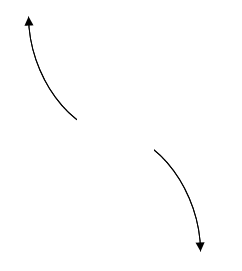
\includegraphics[width=0.3\textwidth]{../Figures/polyEndBehaviorAC.png} & \textbf{B.} 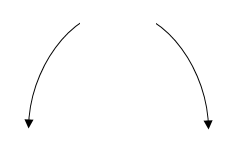
\includegraphics[width=0.3\textwidth]{../Figures/polyEndBehaviorBC.png} \tabularnewline 
\hline 
 & \tabularnewline 
 \textbf{C.} 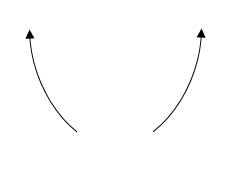
\includegraphics[width=0.3\textwidth]{../Figures/polyEndBehaviorCC.png} & \textbf{D.} 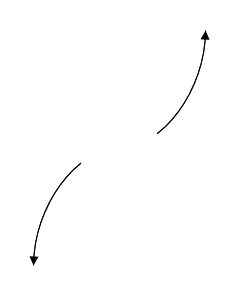
\includegraphics[width=0.3\textwidth]{../Figures/polyEndBehaviorDC.png} \tabularnewline 
\hline 
 E. None of the figures above. & \tabularnewline 
\hline 
 \end{tabular} 
 
\begin{enumerate}[label=\Alph*.] 
\item The function is above the $x$-axis, then passes through.  
\item The function is below the $x$-axis, then touches.  
\item The function is above the $x$-axis, then touches.  
\item The function is below the $x$-axis, then passes through.  
\end{enumerate} 
 
\textbf{General Comment:} \textbf{General Comments:} Remember that end behavior is determined by the leading coefficient AND whether the \textbf{sum} of the multiplicities is positive or negative. 

-----------------------------------------------

2. Construct the lowest-degree polynomial given the zeros below. Then, choose the intervals that contain the coefficients of the polynomial in the form $ax^3+bx^2+cx+d$.
\[ \frac{3}{5}, \frac{2}{5}, \text{ and } \frac{-3}{2} \] 
The solution is $ 50x^{3} +25 x^{2} -63 x + 18 $ 

\begin{enumerate}[label=\Alph*.] 
\item $ a \in [45, 52], b \in [118, 126], c \in [83, 94], \text{ and } d \in [15, 27] $ 

 $50x^{3} +125 x^{2} +87 x + 18$, which corresponds to multiplying out $(5x + 5)(5x + 5)(2x -2)$. 
\item $ a \in [45, 52], b \in [22, 27], c \in [-66, -59], \text{ and } d \in [-25, -16] $ 

 $50x^{3} +25 x^{2} -63 x -18$, which corresponds to multiplying everything correctly except the constant term. 
\item $ a \in [45, 52], b \in [84, 90], c \in [-4, 4], \text{ and } d \in [-25, -16] $ 

 $50x^{3} +85 x^{2} +3 x -18$, which corresponds to multiplying out $(5x + 5)(5x -5)(2x -2)$. 
\item $ a \in [45, 52], b \in [22, 27], c \in [-66, -59], \text{ and } d \in [15, 27] $ 

 * $50x^{3} +25 x^{2} -63 x + 18$, which is the correct option. 
\item $ a \in [45, 52], b \in [-27, -22], c \in [-66, -59], \text{ and } d \in [-25, -16] $ 

 $50x^{3} -25 x^{2} -63 x -18$, which corresponds to multiplying out $(5x + 3)(5x + 2)(2x -3)$. 
\end{enumerate} 
 
\textbf{General Comment:} General Comments: To construct the lowest-degree polynomial, you want to multiply out $(5x -3)(5x -2)(2x + 3)$ 

-----------------------------------------------

3. Construct the lowest-degree polynomial given the zeros below. Then, choose the intervals that contain the coefficients of the polynomial in the form $x^3+bx^2+cx+d$.
\[ 2 + 3 i \text{ and } x -1 \] 
The solution is $ x^{3} -3 x^{2} +9 x + 13 $ 

\begin{enumerate}[label=\Alph*.] 
\item $ b \in [-1.9, 1.3], c \in [-2.08, -1.93], \text{ and } d \in [-3.61, -2.43] $ 

 $x^{3} + x^{2} -2 x -3$, which corresponds to multiplying out $(x -3)(x + 1)$. 
\item $ b \in [2.3, 4.1], c \in [7.06, 9.19], \text{ and } d \in [-13.04, -11.95] $ 

 $x^{3} +3 x^{2} +9 x -13$, which corresponds to multiplying out $(x-(2 + 3 i))(x-(2 - 3 i))(x -1)$. 
\item $ b \in [-3.5, -0.9], c \in [7.06, 9.19], \text{ and } d \in [12.15, 13.07] $ 

 * $x^{3} -3 x^{2} +9 x + 13$, which is the correct option. 
\item $ b \in [-1.9, 1.3], c \in [-1.85, -0.7], \text{ and } d \in [-2.24, -0.56] $ 

 $x^{3} + x^{2} -x -2$, which corresponds to multiplying out $(x -2)(x + 1)$. 
\item $ \text{None of the above.} $ 

 This corresponds to making an unanticipated error or not understanding how to use nonreal complex numbers to create the lowest-degree polynomial. If you chose this and are not sure what you did wrong, please contact the coordinator for help. 
\end{enumerate} 
 
\textbf{General Comment:} Remember that the conjugate of $a+bi$ is $a-bi$. Since these zeros always come in pairs, we need to multiply out $(x-(2 + 3 i))(x-(2 - 3 i))(x-(x -1))$. 

-----------------------------------------------

4. Describe the zero behavior of the zero $x = 3$ of the polynomial below.
\[ f(x) = 7(x - 3)^{9}(x + 3)^{12}(x + 2)^{6}(x - 2)^{10} \] 

 
 The solution is  
 \begin{center} 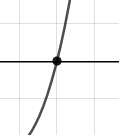
\includegraphics[width=0.3\textwidth]{../Figures/polyZeroBehaviorDC.png} \end{center}\begin{tabular}{|c|c|} 
\hline 
 & \tabularnewline 
 \textbf{A.} 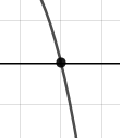
\includegraphics[width=0.3\textwidth]{../Figures/polyZeroBehaviorAC.png} & \textbf{B.} 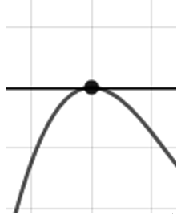
\includegraphics[width=0.3\textwidth]{../Figures/polyZeroBehaviorBC.png} \tabularnewline 
\hline 
 & \tabularnewline 
 \textbf{C.} 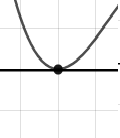
\includegraphics[width=0.3\textwidth]{../Figures/polyZeroBehaviorCC.png} & \textbf{D.} 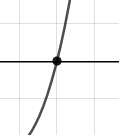
\includegraphics[width=0.3\textwidth]{../Figures/polyZeroBehaviorDC.png} \tabularnewline 
\hline 
 E. None of the figures above. & \tabularnewline 
\hline 
 \end{tabular} 
 
\begin{enumerate}[label=\Alph*.] 
\item   
\item   
\item   
\item   
\end{enumerate} 
 
\textbf{General Comment:} \textbf{General Comments:} You will need to sketch the entire graph, then zoom in on the zero the question asks about. 

-----------------------------------------------

0. Which of the following equations \textit{could} be of the graph presented below?
\begin{center} 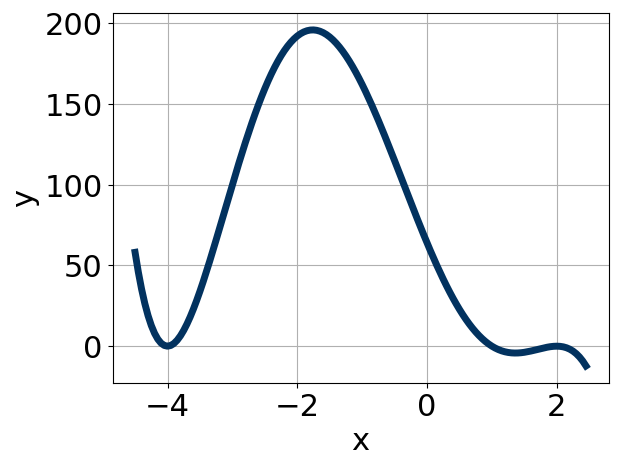
\includegraphics[width=0.3\textwidth]{../Figures/polyGraphToFunctionC.png} \end{center} 

The solution is $ 6x^{10} (x + 3)^{8} (x + 4)^{11} $ 

\begin{enumerate}[label=\Alph*.] 
\item $ 7x^{8} (x + 3)^{5} (x + 4)^{6} $ 

 The factor $(x + 3)$ should have an even power and the factor $(x + 4)$ should have an odd power. 
\item $ 6x^{10} (x + 3)^{8} (x + 4)^{11} $ 

 * This is the correct option. 
\item $ -12x^{6} (x + 3)^{6} (x + 4)^{9} $ 

 This corresponds to the leading coefficient being the opposite value than it should be. 
\item $ -16x^{4} (x + 3)^{10} (x + 4)^{6} $ 

 The factor $(x + 4)$ should have an odd power and the leading coefficient should be the opposite sign. 
\item $ 13x^{10} (x + 3)^{5} (x + 4)^{7} $ 

 The factor $(x + 3)$ should have an even power. 
\end{enumerate} 
 
\textbf{General Comment:} General Comments: Draw the x-axis to determine which zeros are touching (and so have even multiplicity) or cross (and have odd multiplicity). 

-----------------------------------------------


\end{document}

